\documentclass[a4paper]{report}

\usepackage{amssymb, amsmath}
\usepackage{tikz}

\newcommand{\vens}{\ensuremath{v_{\mathrm{ens}}}}

\title{Dimensional Analysis of Perturbation Height}
\author{Nat Lund}

\begin{document}
\maketitle

The highly influential paper ``Achieving large slip with superhydrophobic surfaces: Scaling laws for generic geometries" by Christophe Ybert \emph{et al.} gives several scaling laws.  In the derivation for the first scaling law, they appear to assume that if a surface feature of width $a$ causes a perturbation in the flow that extends a height $d$, then $d$ scales as $a$.

In this appendix we use dimensional analysis to argue that for a flow with a fixed velocity and pressure, then it is indeed true that $d$ scales as $a$.

\vspace*{1em}
The physical situation is that of two-dimensional perturbed plug flow.  The liquid sits on top of a sparse nanograting, so that most of the fluid boundary is a liquid-air interface, which is assumed to have negligible drag (perfect slip).  The ridges of the nanograting have width $a$, and the liquid sticks to the top them (no slip).  The flow is transverse to the ridges, and is very close to plug flow, since the fluid boundary is mostly perfect slip.

The plug-like flow is perturbed by the presence of the no-slip ridges; the perturbation can be considered to be the region where flow is different from pure plug flow to some (arbitrary) degree.  The perturbed region has a perturbation height $d$. 

\begin{center}
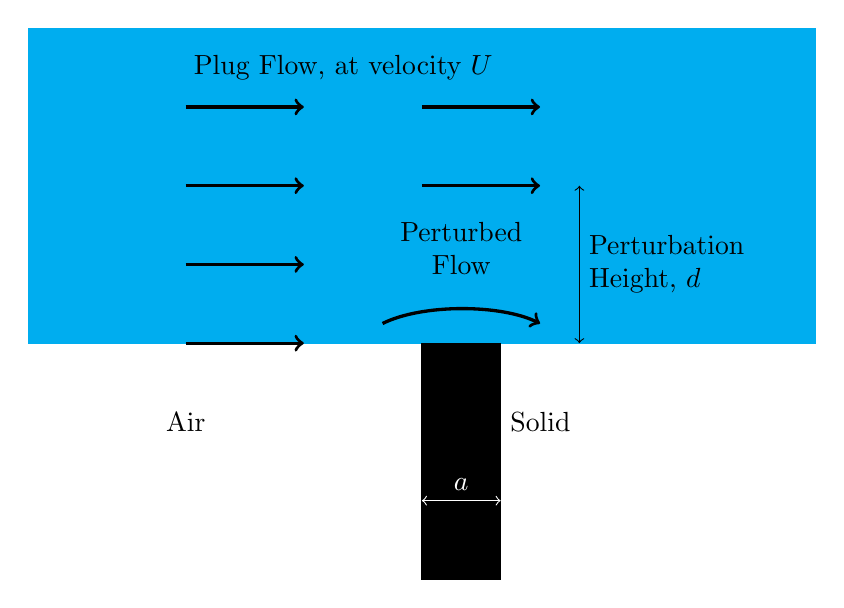
\begin{tikzpicture}

\filldraw[color=cyan] (-5,4) rectangle (5,0);
\filldraw (0,0) rectangle (1,-3);
\node at (-3,-1) {Air};
\node at (1,-1) [right] {Solid};

\draw [color=white, <->] (0,-2) -- node[above] {$a$} (1,-2);

\node at (-1,3.5) {Plug Flow, at velocity $U$};

\foreach \z in {0,1,2,3}
   \draw [->,very thick] (-3, \z) -- (-1.5, \z);
   
\node at (0.5,1.2) [align=center] {Perturbed\\Flow};
\draw [->, very thick] (-0.5,0.25) .. controls (0,0.5) and (1,0.5) .. (1.5, 0.25);
\foreach \z in {2,3}
   \draw [->, very thick] (0, \z) -- (1.5, \z);

\draw [<->] (2,0) -- node[right,align=left]{Perturbation\\Height, $d$} (2,2);


%\filldraw (6.5,0) rectangle +(1,-3);
%\draw [<->](6.5,0) -- node[left] {$d$} +(0,2);
%\draw [->](6.5,2) -- node[above] {$U$} +(2,0);
%\draw [<->](6.5,0) --  +(2,2);
%\node at (7.5,0.7) [right] {$\frac{\partial u}{\partial z} \simeq \frac{U}{d}$};

\end{tikzpicture}
\end{center}

What is perturbation height $d$?

It will be a function of some fundamental physical parameters:
\begin{itemize}
    \item Ridge width $a$
    \item Velocity $U$
    \item Viscosity $\eta$
    \item Density $\rho$
    \item Pressure $p$
\end{itemize}

In other words $d = g(a, U, \eta, \rho, p )$. $\;\;$ Or equivalently, $f(d,a,U,\eta, \rho, p)=0$.
\vspace*{1em}

Physical variables have dimensions:
%\begin{gather*}
%d = [m],\;\; a = [m],\;\; U = [ms^{-1}],\\
% \eta = [kg s^{-1} m^{-1}], \;\; \rho = [kg m^{-3}], \;\;\; p = [kg m^{-1} s^{-2}]
%\end{gather*}
%or
\begin{equation}
d = [m],\;\;\; a = [m],\;\;\; U = \left[\frac{m}{s} \right],\;\;\;
 \eta = \left[\frac{kg}{ms} \right],\;\;\; \rho = \left[\frac{kg}{m^{3}} \right]
 ,\;\;\; p = \left[ \frac{kg}{m s^{2}} \right]
\end{equation}

Units are arbitrary, so it is useful to obtain the height $d$ in terms of the other length scale $a$.  In other words, $d$ and $a$ have some \emph{ratio} that is a dimensionless function of the other physical variables:
\begin{equation}
\frac{d}{a} = \text{Dimensionless} \; f(U, \eta, \rho, p)
\end{equation}

Furthermore, the physical variables will appear as \emph{powers}, multiplied by some constant, or as the argument of functions such as log and cosine.  Those functions are dimensionless, so their arguments must be dimensionless.  Wrapping those functions into the dimensionless variable $C$, we have something like:
\begin{equation}
\frac{d}{a} = C \; U^{w} \eta^{x} \rho^{y} p^{z}
\end{equation}

Now, the physical variables on the right hand side must be in powers such that the units cancel out to be a dimensionless constant.
\begin{gather*}
\text{Constant} = \left[ \frac{m}{s} \right]^{w} \left[ \frac{kg}{ms} \right]^{x}
\left[ \frac{kg}{m^{3}} \right]^{y} \left[ \frac{kg}{m s^{2}} \right]^{z} \\
 = \left[ \frac{m^{w} kg^{x} kg^{y} kg^{z}}{s^{w} m^{x} s^{x} m^{3y} m^{z} s^{2z}} \right] 
 = \left[ \frac{m^{w} kg^{x+y+z}}{m^{x+3y+z} s^{w+x+2z}} \right]
\end{gather*}
\begin{equation}
\text{Constant} = \left[ kg^{x+y+z} m^{w-x-3y-z} s^{-w-x-2z} \right] 
\end{equation}

Thus, the units cancel iff the indices $w,x,y,z$ simultaneously satisfy:
\begin{align}
x+y+z = 0 \\ w-x-3y-z = 0 \\ -w-x-2z = 0 
\end{align}

We can express and solve these three simultaneous equations with matrix algebra.

\begin{equation}
 \begin{bmatrix}
0  &  1 & 1  &  1 \\
1  & -1 & -3 & -1 \\
-1 & -1 & 0  & -2
\end{bmatrix}
\begin{bmatrix}
w \\ x \\ y \\ z \\
\end{bmatrix}
=
\begin{bmatrix}
0 \\ 0 \\ 0 \\ 0 \\
\end{bmatrix}
\end{equation}

Gauss-Jordan reduction:

\begin{equation*} 
\begin{bmatrix}
0  &  1 & 1  &  1 \\
1  & -1 & -3 & -1 \\
-1 & -1 & 0  & -2
\end{bmatrix}
\begin{matrix}
\text{Swap} \\
\text{R1 \& R2} \\
\\
\end{matrix}
\begin{bmatrix}
1  & -1 & -3 & -1 \\
0  &  1 & 1  &  1 \\
-1 & -1 & 0  & -2
\end{bmatrix}
\begin{matrix}
\\
\\
\text{R3 + R1}
\end{matrix}
\begin{bmatrix}
1  & -1 & -3 & -1 \\
0  &  1 & 1  &  1 \\
0 & -2 & -3  & -3
\end{bmatrix} 
\end{equation*}

\begin{equation*}
\begin{matrix}
\\
\\
\text{R3 + 2R2}
\end{matrix}
\begin{bmatrix}
1  & -1 & -3 & -1 \\
0  &  1 & 1  &  1 \\
0  &  0 & -1 & -1
\end{bmatrix}
\begin{matrix}
\text{R1 + R2} \\
\\
\\
\end{matrix}
\begin{bmatrix}
1  &  0 & -2 & 0 \\
0  &  1 & 1  &  1 \\
0  &  0 & -1 & -1
\end{bmatrix}
\begin{matrix}
\\
\text{R2 + R3} \\
\\
\end{matrix}
\begin{bmatrix}
1  &  0 & -2 & 0 \\
0  &  1 & 0  & 0 \\
0  &  0 & -1 & -1
\end{bmatrix}
\end{equation*}

\begin{equation*}
\begin{matrix}
\\
\\
\text{R3 $\times$ -1} \\
\end{matrix}
\begin{bmatrix}
1  &  0 & -2 & 0 \\
0  &  1 & 0  & 0 \\
0  &  0 & 1  & 1
\end{bmatrix}
\begin{matrix}
\text{R1 + 2R3} \\
\\
\\
\end{matrix}
\begin{bmatrix}
1  &  0 & 0  & 2 \\
0  &  1 & 0  & 0 \\
0  &  0 & 1  & 1
\end{bmatrix}
\end{equation*}

Our simultaneous equations have simplified to:
\begin{equation*}
\begin{bmatrix}
1  &  0 & 0  & 2 \\
0  &  1 & 0  & 0 \\
0  &  0 & 1  & 1
\end{bmatrix}
\begin{bmatrix}
w \\ x \\ y \\ z
\end{bmatrix}
=
\begin{bmatrix}
0 \\ 0 \\ 0 \\ 0
\end{bmatrix}
\quad
\Rightarrow
\quad
\begin{matrix}
w + 2z  = 0 \\
x = 0 \\
y + z = 0
\end{matrix}
\quad \text{so} \quad
\begin{matrix}
w = -2z \\ x = 0 \\ y = -z
\end{matrix}
\end{equation*}

As a check, we substitute $w = -2z $, $x=0$ and $ y = -z $ back into
\begin{align*}
x + y + z = 0      & &                  & & 0 + -z +z = 0        & &                 & & 0 = 0 \\
w - x - 3y - z = 0 & & \mathrm{getting} & & -2z + 0 + 3z - z = 0 & & \text{which is} & & 0 = 0 \\
-w - x - 2z = 0    & &                  & & 2z - 0 - 2z = 0      & &                 & & 0 = 0
\end{align*}

%\begin{equation}
%\begin{matrix}
%x+y+z = 0 \\
%w-x-3y-z = 0 \\
%-w-x-2z = 0
%\end{matrix} \;\;\;
%\text{getting} \;\;\;
%\begin{matrix}
%0 + -z + z =0 \\
%-2z + 0 + 3z -z =0\\
%2z - 0 - 2z = 0
%\end{matrix} \;\;\;
%\text{which is} \;\;\;
%\begin{matrix}
%0 = 0 \\
%0 = 0 \\
%0 = 0 \\
%\end{matrix}
%\end{equation}

Hence, our formula must be of the form:
\begin{equation}
\frac{d}{a} = C \; U^{-2z} \eta^{0} \rho^{-z} p^{z}
\end{equation}

Interestingly, our formula is \emph{not} a function of viscosity $\eta$.
For the simplest case of $z=1$, we have:
\begin{equation}
\frac{d}{a} = C \frac{p}{\rho U^2}
\end{equation}

The dimensionless quantity
\begin{equation}
 \frac{\rho U^2}{p} = \frac{[kg m^{-3}] [m s^{-1}]^2}{[kg m^{-1} s^{-2}]} = \frac{[kg m^{-1} s^{-2}]}{[kg m^{-1} s^{-2}]} 
\end{equation}
has the obscure name of the Ruark number.

\vspace*{1em}
But the expressions
\begin{equation}
\frac{d}{a} = C \left( \frac{\rho U^2}{p} \right)^7
\quad \text{or} \quad
\frac{d}{a} = \sqrt{ \frac{\rho U^2}{p} } \cos \left( \frac{\rho U^2}{p} \right)
\end{equation}
would be equally valid.  How can we refine further?

\vspace{1em}
Note that we have explicitly assumed that the ratio $d/a$ is a function of $U, \eta, \rho, p$ \emph{only.} i.e. $d$ and $a$ do not appear on the right hand side. A more complete treatmeat would relax that assumption.  Such a treatment is the Buckingham Pi Theorem.  We shall explore this now.

\pagebreak

\subsection*{Formal Treatment - Buckingham $\pi$ Theorem }

Assume there is a physical relationship that can be expressed as $f(a,\rho ,U,\eta, p, d) = 0 $.
Formally, there are 6 dimensional variables, and 3 physical units.
So if $f$ \emph{expresses a valid physical law,} there will be 
6 - 3 = 3 dimensionless variables, $\pi_1$, $\pi_3$ and $\pi_2$.
Then $f$ can be expressed as:
\begin{equation}
\Phi (\pi_1,\pi_2,\pi_3) = 0
\end{equation}

%We suspect
%\begin{equation*}
%\pi_1 = \frac{d}{a}, \quad \pi_2 = \frac{\rho U^2}{p}, \quad \pi_3 = \eta^0 = 1
%\end{equation*}
%
%
%Then $f(a,\rho ,U,\eta, p, d) = 0 $ would be equivalent to  $\Phi(\pi_1, \pi_2)=0$, which we have found to be
%\begin{equation*}
%\pi_1 - C \pi_2 = 0
%\end{equation*}
%Let us find out.
%\vspace{1em}

The relations between physical variables and dimensions are expressed in the dimensional matrix $M$:

\begin{center}
\begin{tabular}{l l l l l l l }
   & $a$ & $\rho$ & $U$ & $\eta$ & $p$  & $d$ \\
m  & 1   &  -3    &  1  &   -1   &  -1  & 1  \\
kg & 0   &  1     &  0  &    1   &  1   & 0  \\
s  & 0   &  0     &  -1 &   -1   &  -2  & 0  \\
\end{tabular}
\end{center}

The components of the dimensional matrix $M$ are the exponents on the fundamental units.  The components of a vector $\vec{x}$ are the exponents of the physical variables.  The simultaneous equations that express the constraint that the physical formula be dimensionless are expressed as:
\begin{equation}
M \vec{x} = 0
\end{equation}
We are solving for the appropriate exponents on the physical variables that satisfy the non-dimensionality requirement.

However, there will be a whole \emph{family} of solutions. They form a space; the set of all $\vec{x}$ satisfying $M\vec{x}= 0$.  The set is known as the \emph{null space} or \emph{kernel} of $M$.  We would like a basis for the space.  The basis vectors will represent the dimensionless variables $\pi_1,\pi_2, \pi_3$; they will be things like the Reynolds number.

\subsubsection*{Basis of Nullspace from Column Echelon Form}

To find a basis for the null space of $M$, we use the following technique:
Glue the identity matrix $I$ underneath $M$.  Transpose the result, forming a new matrix $A$.  Row reduce $A$ until the part corresponding to $M$ is in row echelon form.  Then, the basis vectors are: any row of $I$ with all zeros in the corresponding row of $M$.

Here goes:

\begin{equation*} 
\begin{bmatrix}
1  & -3  &  1  & -1  & -1  &  1  \\
0  &  1  &  0  &  1  &  1  &  0  \\
0  &  0  & -1  & -1  & -2  &  0 \\
\hline
1  &  0  &  0  &  0  &  0  &  0 \\ 
0  &  1  &  0  &  0  &  0  &  0 \\ 
0  &  0  &  1  &  0  &  0  &  0 \\ 
0  &  0  &  0  &  1  &  0  &  0 \\ 
0  &  0  &  0  &  0  &  1  &  0 \\ 
0  &  0  &  0  &  0  &  0  &  1 \\ 
\end{bmatrix}^T
=
\begin{bmatrix}
1  &  0  &  0  &  1  &  0  &  0  &  0  &  0  &  0 \\
-3 &  1  &  0  &  0  &  1  &  0  &  0  &  0  &  0 \\
1  &  0  & -1  &  0  &  0  &  1  &  0  &  0  &  0 \\
-1 &  1  & -1  &  0  &  0  &  0  &  1  &  0  &  0 \\
-1 &  1  & -2  &  0  &  0  &  0  &  0  &  1  &  0 \\
1  &  0  &  0  &  0  &  0  &  0  &  0  &  0  &  1
\end{bmatrix}
\end{equation*}

\begin{equation*}
\begin{matrix}
\\
\text{R3 + 3R1}\\
\text{R3 - R1} \\
\text{R4 + R1} \\
\text{R5 + R1} \\
\text{R6 - R1}
\end{matrix}
\begin{bmatrix}
1  &  0  &  0  &  1  &  0  &  0  &  0  &  0  &  0 \\
0  &  1  &  0  &  3  &  1  &  0  &  0  &  0  &  0 \\
0  &  0  & -1  & -1  &  0  &  1  &  0  &  0  &  0 \\
0  &  1  & -1  &  1  &  0  &  0  &  1  &  0  &  0 \\
0  &  1  & -2  &  1  &  0  &  0  &  0  &  1  &  0 \\
0  &  0  &  0  & -1  &  0  &  0  &  0  &  0  &  1
\end{bmatrix}
\end{equation*}

\begin{equation*}
\begin{matrix}
\\
\\
\text{R3 $\times$ -1} \\
\text{R4 - R2} \\
\text{R5 - R2} \\
\\
\end{matrix}
\begin{bmatrix}
1  &  0  &  0  &  1  &  0  &  0  &  0  &  0  &  0 \\
0  &  1  &  0  &  3  &  1  &  0  &  0  &  0  &  0 \\
0  &  0  &  1  &  1  &  0  & -1  &  0  &  0  &  0 \\
0  &  0  & -1  & -2  & -1  &  0  &  1  &  0  &  0 \\
0  &  0  & -2  & -2  & -1  &  0  &  0  &  1  &  0 \\
0  &  0  &  0  & -1  &  0  &  0  &  0  &  0  &  1
\end{bmatrix}
\end{equation*}

\begin{equation*}
\begin{matrix}
\\
\\
\\
\text{R4 + R3} \\
\text{R5 + 2R3} \\
\\
\end{matrix}
\begin{bmatrix}
1  &  0  &  0  &  1  &  0  &  0  &  0  &  0  &  0 \\
0  &  1  &  0  &  3  &  1  &  0  &  0  &  0  &  0 \\
0  &  0  &  1  &  1  &  0  & -1  &  0  &  0  &  0 \\
0  &  0  &  0  & -1  & -1  & -1  &  1  &  0  &  0 \\
0  &  0  &  0  &  0  & -1  & -2  &  0  &  1  &  0 \\
0  &  0  &  0  & -1  &  0  &  0  &  0  &  0  &  1
\end{bmatrix}
\end{equation*}

At this point we can stop; the part corresponding to $M$ (the left three columns) is in row echelon form, with the bottom three rows consisting entirely of zeros.  Therefore, the three basis vectors are the bottom three rows of what was the identity matrix:
\begin{equation*}
\begin{bmatrix}
-1 & 0 & 0 & 0 & 0 & 1
\end{bmatrix}
,\;\;
\begin{bmatrix}
0 & -1 & -2 & 0 & 1 & 0
\end{bmatrix}
,\;\;
\begin{bmatrix}
-1 & -1 & -1 & 1 & 0 & 0
\end{bmatrix}
\end{equation*}
whose components are the exponents of our physical variables
\begin{equation*}
\begin{bmatrix}
a & \rho & U & \eta & p & d
\end{bmatrix}
\end{equation*}

We are free to take the \emph{negative} of the basis vectors.  If we do this, then the corresponding dimensionless variables appear in the convenient form:
\begin{equation}
 \pi_1 = \frac{d}{a}, \quad \pi_2 = \frac{\rho U^2}{p}, \quad
 \pi_3 = \frac{\rho a U}{\eta}
\end{equation}


Then, the dimensionless number
\begin{equation*}
\pi_3 = \frac{\rho a U}{\eta} = \frac{[kg m^{-3}] [m] [m s^{-1}]}{[kg m^{-1} s^{-1}]} = \frac{[kg m^{-1} s^{-1}]}{[kg m^{-1} s^{-1}]} = 1
\end{equation*}
is the familiar \emph{Reynolds} number, while $\pi_2 = \frac{\rho U^2}{p}$ is the more obscure \emph{Ruark} number.

\vspace{1em}
(The three vectors \emph{are} linearly independent -- none can be obtained by a linear combination of the other two, since each contains a unique physical variable (specifically $d$, $p$ and $\eta$ ).
But $\pi_3$ is coupled to the other two; in some physical sense, the variables are not independent.)

\vspace{2em}

So while our naive treatment showed that $d/a$ is a function of the Ruark number, the full Buckingham Pi theorem shows that there is a \emph{third} possible dimensionless variable, the Reynolds number:
\begin{equation*}
\pi_1 = \frac{d}{a}, \quad \pi_2 = \frac{\rho U^2}{p}, \quad
 \pi_3 = \frac{\rho a U}{\eta}
\end{equation*}
Note that these are not the \emph{only} possible basis vectors for the nullspace of $M$.  One could even use the dreaded Gram-Schmidt procedure to get an orthonormal basis.  But any basis can be expressed in terms of the basis we have found here.  Therefore, any formula $\Phi(\pi_1, \pi_2, \pi_3)=0$ (for any basis $\pi_1,\pi_2,\pi_3$) can be rewritten so that the ratio $d/a$ appears as a variable, and can be rearranged to:
\begin{gather}
\frac{d}{a} = \Phi(Ru, Re )
\\
\text{where} \quad  Ru = \frac{\rho U^2}{p}, \quad Re = \frac{\rho a U}{\eta}
\end{gather}

\subsubsection*{Conclusion}
The ratio $d/a$ is an unknown function of the Ruark number and the Reynolds number.  Therefore:

\vspace*{1em}
In a series of experiments with a fluid of constant density and viscosity,\\
\textbf{for fixed velocity and pressure,} perturbation height $d$ scales as anomaly width $a$.

\vspace{1em} 
Note that the ratio $d/a$ is not fixed, so $d$ is not \emph{determined} by $a$.  If $a$ is fixed, then $d$ may change as a function of $U, \rho, p$ etc.

\end{document}







\pagebreak

\subsubsection*{Addendum: Orthogonalize Basis Vectors?}
The basis vectors are not orthogonal.  Does it help to orthogonalize?

The most physically meaningful dimensionless variable is the ratio $d/a$.  So we choose to keep $\pi_1$, and orthogonalize based on that.

\subsubsection*{Dreaded Gram-Schmidt Orthogonalization}
\[ \vec{v}_1 = (1, 0,0,0,0,-1),\;\;\; \vec{v}_2 = (0,1,2,0,-1,0),\;\;\;
\vec{v}_3 = (1,1,1,-1,0,0) \]

\[ \vec{u}_1 = \vec{v}_1 \]

\[ \vec{u}_2 = \vec{v}_2 - \frac{\vec{u}_1 \cdot \vec{v}_2}{\vec{u}_1 \cdot \vec{u}_1} \vec{u}_1 = \vec{v}_2 - 0 = \vec{v}_2 \]

\[ \vec{u}_3 = \vec{v}_3 - \frac{\vec{u}_1 \cdot \vec{v}_3}{\vec{u}_1 \cdot \vec{u}_1} \vec{u}_1  -  \frac{\vec{u}_2 \cdot \vec{v}_3}{\vec{u}_2 \cdot \vec{u}_2} \vec{u}_2 \]

\[ = (1,1,1,-1,0,0) - \frac{1}{1+1}(1, 0,0,0,0,-1) - \frac{1+2}{1+4+1}(0,1,2,0,-1,0) \]
\[ = (1,1,1,-1,0,0) - (1/2, 0,0,0,0,-1/2) - (0,1/2,1,0,-1/2,0) \]
\[ = (1/2, 1/2, 0, -1, 1/2, 1/2) \]
Multiplying by 2 gives a parallel vector that is still orthogonal:
\[ \vec{u}_3 = (1,1, 0,-2,1, 1)\]
Three orthogonal vectors. Check:
\[(1,0,0,0,0,-1)\cdot(1,1,0,-2,1,1) = 1-1 = 0 \] 
\[ (0,1,2,0,-1,0)\cdot(1,1,0,-2,1,1) = 1-1 = 0 \]

Recall the physical variables:
\[
\begin{bmatrix}
a & \rho & U & \eta & p & d
\end{bmatrix}
\]

So:
\[ \pi_1 = \frac{d}{a},\;\;\; \pi_2 = \frac{\rho U^2}{p},\;\;\;
 \pi_3 = \frac{a \rho p d}{\eta^2} \]


Check that $\pi_3$ is dimensionless:
\[ \pi_3 = \frac{a \rho p d}{\eta^2} = 
\frac{[m][kg m^{-3}][kg m^{-1}s^{-2}][m]}{[kg m^{-1}s^{-1}]^2} 
= \frac{[kg^2 m^{-2} s^{-2}]}{[kg^2 m^{-2} s^{-2}]} = 1 \]

We have three orthogonal dimensionless variables.  But they are still coupled -- can you vary one without affecting the others?  $\pi_1$ and $\pi_2$ are independent in that sense, but $\pi_3$ causes trouble.  Does this matter? Is there a justification for saying that $\pi_3$ must appear to the zeroth power, i.e. vanish?

\end{document}

\vspace{5em}

\subsubsection*{Basis of Null Space found `by hand'}
As an exercise, we solve $ M \underline{x} = 0$ via Gauss-Jordan reduction.

\[ 
\begin{bmatrix}
1  & -3  &  1  & -1  & -1  &  1  \\
0  &  1  &  0  &  1  &  1  &  0  \\
0  &  0  & -1  & -1  & -2  &  0  
\end{bmatrix}
\begin{matrix}
\text{R1 + 3R2} \\ \\ \\
\end{matrix}
\begin{bmatrix}
1  &  0  &  1  &  2  &  2  &  1  \\
0  &  1  &  0  &  1  &  1  &  0  \\
0  &  0  & -1  & -1  & -2  &  0  
\end{bmatrix}
\]
\[
\begin{matrix}
\text{R1 + R3} \\ \\ \\
\end{matrix}
\begin{bmatrix}
1  &  0  &  0  &  1  &  0  &  1  \\
0  &  1  &  0  &  1  &  1  &  0  \\
0  &  0  & -1  & -1  & -2  &  0  
\end{bmatrix}
\begin{matrix}
\\ \\ \text{R3 $\times$ -1}
\end{matrix}
\begin{bmatrix}
1  &  0  &  0  &  1  &  0  &  1  \\
0  &  1  &  0  &  1  &  1  &  0  \\
0  &  0  &  1  &  1  &  2  &  0  
\end{bmatrix}
\]

Letting $\hat{d}, \hat{\rho}, \hat{U}, \hat{\eta}, \hat{p}, \hat{a}$ stand for the exponents of
$d, \rho, U, \eta, p, a$ respectively, we have:

\[
\begin{bmatrix}
1  &  0  &  0  &  1  &  0  &  1  \\
0  &  1  &  0  &  1  &  1  &  0  \\
0  &  0  &  1  &  1  &  2  &  0  
\end{bmatrix}
\begin{bmatrix}
\hat{d} \\ \hat{\rho} \\ \hat{U} \\ \hat{\eta} \\ \hat{p} \\  \hat{a}
\end{bmatrix}
=
\begin{bmatrix}
0 \\ 0 \\ 0 \\ 0 \\ 0 \\ 0
\end{bmatrix}
\]

By inspection, a kernel vector of $M$ is:
\[
\begin{bmatrix}
1 \\ -1 \\ -2 \\ 0 \\ 1 \\ -1
\end{bmatrix}
\;\;\;
\begin{matrix}
\text{expressible as the sum of} \\ \text{two orthogonal vectors}
\end{matrix}
\;\;\;
\begin{bmatrix}
1 \\ 0 \\ 0 \\ 0 \\ 0 \\ -1
\end{bmatrix}
+
\begin{bmatrix}
0 \\ -1 \\ -2 \\ 0 \\ 1 \\ 0
\end{bmatrix}
\]

The two orthogonal vectors give us:
\[ \pi_1 = \frac{d}{a},\;\;\; \pi_2 = \frac{p}{\rho U^2} \]


\vspace{2em}
Can we cancel the $\eta$ on algebraic grounds?
\[
\begin{matrix}
\hat{d} + \hat{\eta} + \hat{a} = 0 \\
\hat{\rho} + \hat{\eta} + \hat{p} = 0 \\
\hat{U} + \hat{\eta} + 2 \hat{p} = 0 
\end{matrix}
\]

Hmmmm.... $- \hat{\eta} = \hat{U} + 2\hat{p}$ and $-\hat{\eta} = \hat{\rho} + \hat{p}$.  Therefore, $\hat{U} + 2\hat{p} = \hat{\rho} + \hat{p}$, so $\hat{U} + \hat{p} = \hat{\rho}$. Errrr...


\end{document}